\section*{Généralités}
\label{sec:generalites}
\addcontentsline{toc}{section}{Généralités}

\subsection*{Les examens professionnels}
\label{subsec:examsprofs}
\addcontentsline{toc}{subsection}{Les examens professionnels}
\captionsetup{justification=centering}
Bien souvent, les examens professionnels sont l'une des premières choses dont l'on entend parler lorsqu'il est question d'actuariat. Il y a beaucoup d'informations disponibles sur le sujet, autant à partir de sources officielles que sur différents forums de discussion.\vspace{\baselineskip}

Afin d'avoir une bonne idée du cheminement, je vous suggère de vous référer en premier lieu aux informations se trouvant sur les sites des deux principales organisations professionnelles en actuariat: la \href{https://soa.org/member/}{\emph{Society of Actuaries (SOA)}} et la \href{http://www.casact.org/}{\emph{Casualty Actuarial Society (CAS)}}. Essentiellement, ce sont leurs champs d'activité différents qui distinguent ces deux organisations; la CAS se spécialise dans l'assurance IARD, alors que la SOA regroupe les branches investissement, gestion de risques en entreprise, assurance-vie, retraite et assurance-maladie.\footnote{ Il est à noter que la spécialisation \emph{General Insurance} de la SOA n'est pas reconnue par l'Institut canadien des actuaires (ICA).}\vspace{\baselineskip}

Vous remarquerez qu'il y a, autant du côté de la CAS que de la SOA, une série d'examens préliminaires suivie par des examens avancés. Certains examens préliminaires sont communs à tous, peu importe la spécialisation que l'on désire atteindre. Ces examens sont P/1, FM/2, IFM/3F et LTAM/4. La raison pour laquelle il y a deux appelations par examen préliminaire est que la SOA et la CAS ne nomment pas de la même façon ces examens dans leur cheminement. Du côté de la SOA, on a les examens P, FM, IFM et STAM, alors que ces mêmes examens se nomment 1, 2, 3F et 4 du côté de la CAS. La section \nameref{sec:prelims} du présent document parlera plus en détails du contenu de ces examens, du matériel d'étude à utiliser et des façons de bien s'y préparer.\vspace{\baselineskip}

Il y a énormément d'informations sur les sites de la SOA et de la CAS, mais ils ne disent pas tout non plus. La SOA parle souvent  d'une \emph{règle du pouce} d'environ 100 heures d'étude par heure d'examen, sans donner de détails vraiment sur la façon de répartir ces heures ou quel matériel d'étude utiliser par exemple. Les différents forums de discussion sont une excellente ressource pour connaître ce genre d'informations. Les deux principaux étant \href{http://www.actuarialoutpost.com/}{\emph{Actuarial Outpost}} et \href{https://www.reddit.com/r/actuary}{\emph{/r/actuary}}. La page \href{https://www.reddit.com/r/actuary/wiki/index#wiki_the_frequently_asked_questions_.28faqs.29}{\emph{FAQ}} de \emph{/r/actuary} contient beaucoup d'informations utiles pour les gens qui débutent en actuariat. Également, la discussion \href{https://www.reddit.com/r/actuary/comments/1enzdd/how_long_to_get_to_asa_is_two_years_possible/}{\emph{How long to get to ASA}} de ce même site contient des réponses intéressantes au sujet du temps nécessaire pour compléter les examens. \vspace{\baselineskip}

Pour connaître des statistiques au sujet des examens professionnels, vous pouvez consulter le site \href{http://actuarial-lookup.com/}{\emph{actuarial-lookup}}. Ce site contient des données de 2007 jusqu'à aujourd'hui.

\begin{center}
\begin{figure}[hp]
% \textbf{Your title}\par\medskip
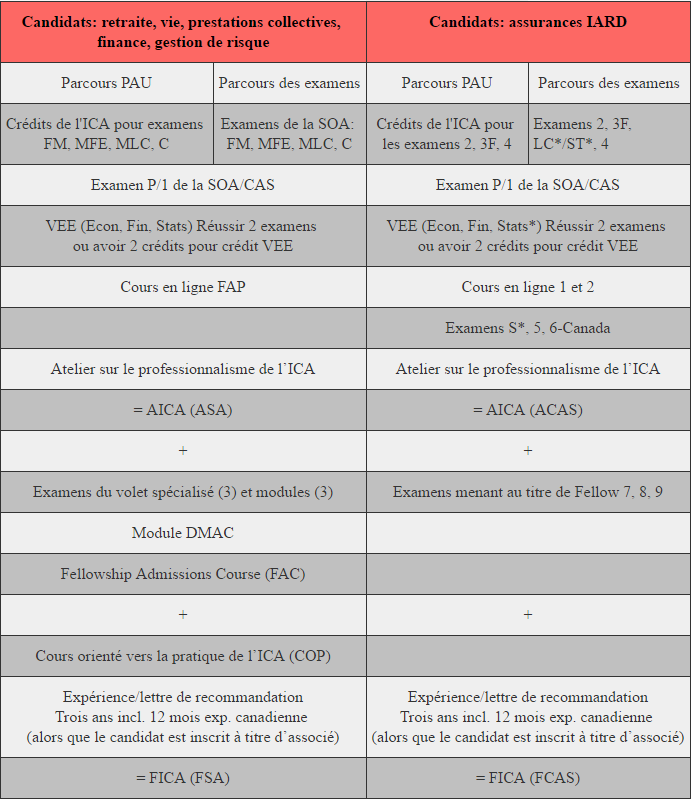
\includegraphics[width=0.92\textwidth]{tableau_ICA.png}
\caption{Cheminement professionnel en actuariat --- Grille fournie par Joseph Gabriel de l'Institut canadien des actuaires}
\end{figure}
\par
\end{center}

Note: Les examens MAS-1 et MAS-2 remplacent les examens S et C respectivement pour les candidats de la CAS. Les examens IFM, LTAM et STAM remplacent les examens MFE, MLC et C respectivement pour les candidates de la SOA. Les examens SRM et PA sont quant à eux des ajouts pour les candidats de la SOA.\vspace{\baselineskip}

Vous trouverez l'information quant aux cours qui permettent d'obtenir les accréditations d'examen de l'ICA dans votre \href{https://www.act.ulaval.ca/programmes-et-cours/premier-cycle/guide-de-letudiant/}{guide de l'étudiant}. Cette information se trouve généralement dans les dernières pages du document. Il est important de savoir que la CAS reconnaît les accréditation de l'ICA, mais que la SOA ne les reconnaît pas. Ainsi, un candidat qui obtient des accréditations pour certains examens peut obtenir les titres de Fellow de l'ICA et de la CAS mais, s'il est du côté de la SOA, il ne pourra pas devenir Fellow de la SOA --- il sera seulement Fellow de l'ICA.

\subsection*{Les crédits VEE}
\label{subsec:vee}
\addcontentsline{toc}{subsection}{Les crédits VEE}
Les crédits VEE (\emph{Validation by Educational Experience}) sont une composante nécessaire pour obtenir le titre d'Associé. Les VEE permettent de couvrir des sujets qui ne sont pas formellement testés lors des examens préliminaires. La CAS et la SOA ont deux VEE en commun: le VEE \emph{Corporate Finance and Accounting} et le VEE \emph{Economics}. La SOA compte également le VEE \emph{Applied Statistical Methods}. Anciennement, la CAS comptait également ce troisième VEE, mais ils ont décidé de l'enlever suite à la création de l'Examen S (maintenant MAS-1).\vspace{\baselineskip}

Les crédits VEE peuvent être complétés en obtenant une note d'au moins B- dans certains cours du baccalauréat. Présentement, les cours qui permettent d'obtenir le VEE \emph{Corporate Finance and Accounting} sont \textit{ACT-1006 Gestion du risque financier I} \textbf{et} \textit{CTB-1000 Comptabilité générale} (la partie Accounting du VEE devient nécessaire après le 1er Juillet 2018), alors que les cours qui permettent de compléter le VEE \emph{Economics} sont \textit{ECN-1000 Principes de microéconomie} \textbf{et} \textit{ECN-1010 Principes de macroéconomie}. Du côté de la SOA, on peut également obtenir le crédit VEE \emph{Applied Statistical Methods} avec une cote supérieure ou égale à B- dans le cours \textit{ACT-2000 Analyse statistique des risques actuariels} (entre en vigueur le 1er Juillet 2018. Anciennement, c'était les cours \textit{ACT-2003 Modèles linéaires en actuariat} \textbf{et} \textit{ACT-2010 Séries chronologiques} qui procuraient le VEE. Pour ceux qui auraient des questions sur la transition, n'hésitez pas à nous contacter). Advenant le cas où vous n'auriez pas la cote minimale pour obtenir le crédit, vous devrez éventuellement compléter un cours en ligne sur le sujet du VEE en question, lequel sera suivi d'un examen.

\newpage

\subsection*{Alternatives et compléments aux manuels}
\label{subsec:alternatives}
\addcontentsline{toc}{subsection}{Alternatives et compléments aux manuels}
Il existe quelques alternatives et compléments aux manuels d'étude qui ont été présentés ci-dessus. Par exemple, les sites \href{http://www.theinfiniteactuary.com/}{\emph{The Infinite Actuary}} et \href{https://www.coachingactuaries.com/}{\emph{Coaching Actuaries}} offrent des formations préparatoires sous forme de vidéos pour tous les examens préliminaires (et certains examens avancés dans le cas de \emph{The Infinite Actuary}). Ces ressources sont toutefois peu populaires auprès des étudiants du baccalauréat, puisqu'elles sont souvent dispendieuses.\vspace{\baselineskip}

Un complément incontournable aux manuels d'étude est le système dynamique de génération d'examens ADAPT. Ce système est offert par le site \href{https://www.coachingactuaries.com/}{\emph{Coaching Actuaries}} et comporte une énorme banque de questions pour chacun des examens préliminaires. Le fonctionnement de ADAPT est plutôt simple; on débute au niveau 0, le système génère des examens pour vous et, dépendamment de votre résultat à l'examen, votre niveau (\emph{Earned Level} en anglais) va augmenter. Le niveau de l'examen correspond à sa difficulté; plus il est élevé, plus il sera difficile. Vous pourrez également plus facilement voir quelles sont les sections de l'examen où vous avez le plus de difficulté et créer des quiz spécifiquement sur ces sections afin de vous améliorer. L'objectif est d'atteindre un niveau 7 (sans tricher --- évidemment), puisque les statistiques disponibles montrent qu'environ 90\% des gens qui ont atteint ce niveau ont réussi leur examen. Vous aurez aussi droit à un rabais de 20\% pour les examens P, FM, IFM (MFE) grâce au code LAVALPC20 et un rabais de 30\% pour les examens C (STAM/MAS-2), MLC (LTAM), S (MAS-1) grâce au code LAVALPC30. Voir ce \href{https://www.youtube.com/watch?v=ZBxLa2J5jhs}{vidéo} pour une brève présentation de ADAPT.

\newpage